\chapter{Theoretical Framework}
\label{sec:framework}
The previous two chapters have given a theoretical overview of the \acl{SM} and
\acl{SUSY}. In order to bring the predictions of these theories closer to the
realm of experiment, this chapter will provide a higher-level discussion more
suited to the results that will be presented later on.

A brief account of vector boson production at a hadron collider is given in
\sec~\ref{sec:framework_wpol}, along with details of the polarisation of \PW
bosons at the \ac{LHC}. This motivates the measurement described in
\chap~\ref{sec:wpol} and forms the framework within which the experimental
results will be interpreted.

For the supersymmetry search, several possible models are discussed in
\sec~\ref{sec:framework_susy}. Given the unknown nature of \ac{SUSY}, these
models have informed the design of the search to only a limited extent. However,
they are highly relevant to \chap~\ref{sec:interpretation}, where the results
of the \ac{SUSY} search will be interpreted in the context of these models.

\section[W Polarisation]{\PW Polarisation}
\label{sec:framework_wpol}
Some theoretical background relating to the \acl{SM} has been presented in
\sec~\ref{sec:sm}.  Here, \PW and \PZ production in association with jets at
hadron colliders -- abbreviated respectively as \Wjets and \Zjets -- will be
briefly explained. Theoretical background to the \PW polarisation will then be
discussed.

\subsection{Vector Boson Production at Hadron Colliders}
\label{sec:framework_vboson}
A detailed account of massive vector boson production at hadron colliders can be
found in~\cite{nadolsky, pink_book}. Production at hadron colliders proceeds
predominantly via $\Pquark\APquark$ or $\Pquark\Pgluon$ interactions and is
highly dependent on \ac{QCD} calculations. Cross-sections can be calculated as
the product of the hard scattering cross-section evaluated in perturbative
\ac{QCD} and a \ac{PDF}. The \ac{PDF} is a probability density function for the
probability of finding a parton with a given fraction of the longitudinal
momentum, $x$, as a function of the momentum transfer, $Q^2$. It is obtained
from a fit of a parameterised model to hadronic data. Cross-section calculations
for these processes may be referred to as \ac{LO} or \ac{NLO} indicating the
precision of the calculation in terms of the expansion of the strong coupling
constant, \alphas~\cite{ellis_wp3jet}.

These processes have been extensively studied and significant recent progress
made, particularly for calculation of higher jet multiplicity
observables~\cite{berger_left_handed_w,berger_nlo_qcd_wjet}. The \Wjets
cross-section has been calculated at \ac{NLO} for up to 4
jets~\cite{berger_wp4jet}. The discussion will now turn to aspects relevant to
\Wjets production and in particular the polarisation effects.

\subsection{Polarisation Effects Parallel to the Beam Line}
For small values of \PW transverse momentum, \PtW, the differential angular
cross-section for the process
$\Pp\Pp\longrightarrow\PWpm\longrightarrow\Plpm\Pgnl$ follows the Drell-Yan
distribution:
\begin{equation*}
\frac{dN}{d(\cos\theta)} \propto (1\mp \cos\theta)^2.
\end{equation*}

It is well known from straightforward helicity arguments~\cite{mirkes_w_1994}
that \PW bosons produced along the beam axis will exhibit a 100\% left-handed
polarisation. This can be seen by considering the leading order partonic
subprocesses:
\begin{equation*}
\Pup\APdown \longrightarrow \PWp \qquad\textrm{and}\qquad
\Pdown\APup\longrightarrow\PWm.
\end{equation*}
Firstly, note that in the case of valence quarks, the fraction of the proton
momentum carried by the quark (as determined by the \aclp{PDF}) is greater than
that of the anti-quark. In addition given that the \ac{LHC} is a $\Pp\Pp$
collider, valence anti-quarks are not present. Anti-quarks must be drawn from
the sea and are therefore likely to be low momentum. Taking these two facts
together, the quark is very likely to have higher momentum than the
anti-quark. By momentum conservation, it is expected that the \PW will be
produced overwhelmingly in the direction of the original quark. Then given the
\VminusA nature of the weak interaction (see \sec~\ref{sec:sm_electroweak}, it
is seen that the quark must be left-handed and, by helicity conservation the \PW
will be polarised nearly 100\% left-handedly along the beam axis. A small
dilution will occur in instances where the anti-quark has by chance a larger
momentum fraction than the quark.

It is worth mentioning that the situation is not identical at the Tevatron
$\Pp\Pap$ collider. Although the \PWp also possess a 100\% left-handed
polarisation along the beam-line (via similar arguments to those given above),
the \PWm are found to have a near 100\% right-handed polarisation. This is a
result of the subprocess $\APup\Pdown\longrightarrow\PWm$ where this time the
\APup carries more momentum.

% TODO: Mention the effect this has on the rapidity distribution

\subsection{Polarisation Effects in the Transverse Plane}
\label{sec:polarisation}
In the case, where the \PW boson carries a significant transverse momentum, the
situation is more complex. In general, the \PW may be produced in association
with a number of jets. For the sake of this discussion we will consider cases
involving only a single jet. Also, in order to simplify matters, one need only
consider the \PWp case as the \PWm case is very similar. At leading order, three
subprocesses should be considered~\cite{berger_left_handed_w},
\begin{equation}
\label{eqn:w1jet_processes}
\Pup\Pgluon\longrightarrow\PWp\Pdown\;\textrm{,} \qquad
\Pup\APdown\longrightarrow\PWp\Pgluon\qquad\textrm{and} \qquad
\Pgluon\APdown\longrightarrow\PWp\APup.
\end{equation}
For sufficiently large \PtW, the soft gluon enhancement of
$\Pup\APdown\longrightarrow\PWp\Pgluon$ and the quark-gluon subprocess is found
to dominate. It has been found that 70-80\% of $\PW+N$~jet ($N \leq 4$)
production at \ac{LO} is initiated by this subprocess.

Considering the quark-gluon subprocess, the $s$ and $t$ channel diagrams are
shown in \fig~\ref{fig:w1jet_st}. For the $s$ channel diagram, the on-shell
\Pdown quark is directly coupled to the \PW and therefore must be in a negative
helicity state (i.e. left-handed). Assuming a positive helicity for the W boson
(as depicted in \fig~\ref{fig:w1jet_st_s}), the spin along the $\PW\Pdown$
axis is $1+\frac{1}{2} = \frac{3}{2}$. Such a configuration is not allowed for
the \spinhalf off-shell quark and thus the $s$-channel diagram should lead to a
100\% left-handed polarisation of the \PW. In contrast, the $t$ channel diagram
is not similarly constrained by spin arguments (since the \PW is not coupled
directly to the quark) and thus the polarisation will not be seen.

It can be shown that for a left-handed incoming gluon, the $t$-channel diagram
can be made to vanish~\cite{berger_left_handed_w}. For a right-handed gluon, the
\PW polarisation is not constrained but has been shown to become predominantly
right-handed at high \PtW. At high \PtW, the outgoing \PW helicity will be
almost 100\% correlated with the incoming gluon and due to a factor 4 difference
in the size of the corresponding matrix elements, the \PW is expected to
asymptotically approach an 80\% left-handed polarisation with increasing
\PtW. Due to the \VminusA coupling, the decay leptons may act as an analyser of
the \PW polarisation. Having provided some motivation for the existence of the
effect, a more detailed discussion will follow.

\begin{figure}
\centering
\subfloat[]{\label{fig:w1jet_st_s}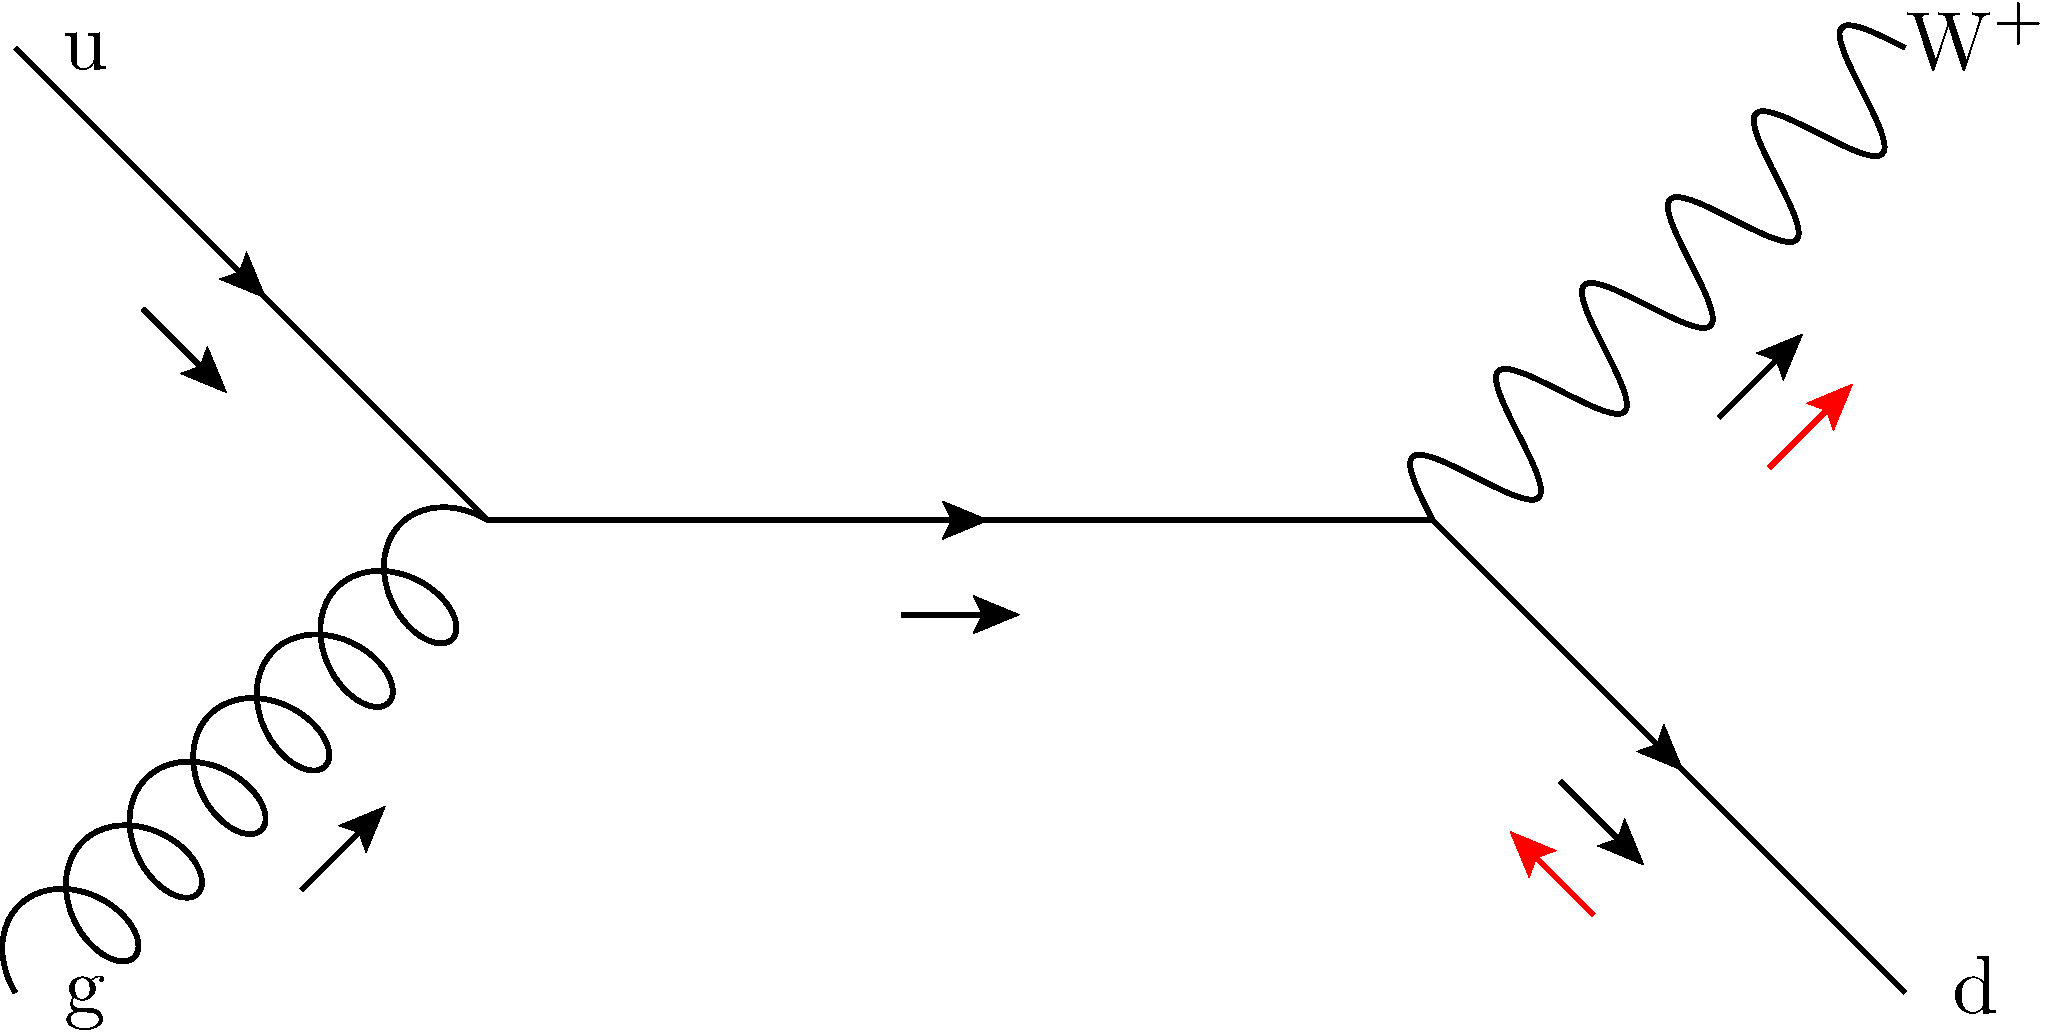
\includegraphics[width=0.5\textwidth]{fig/wpol_1jet_s}}\quad
\subfloat[]{\label{fig:w1jet_st_t}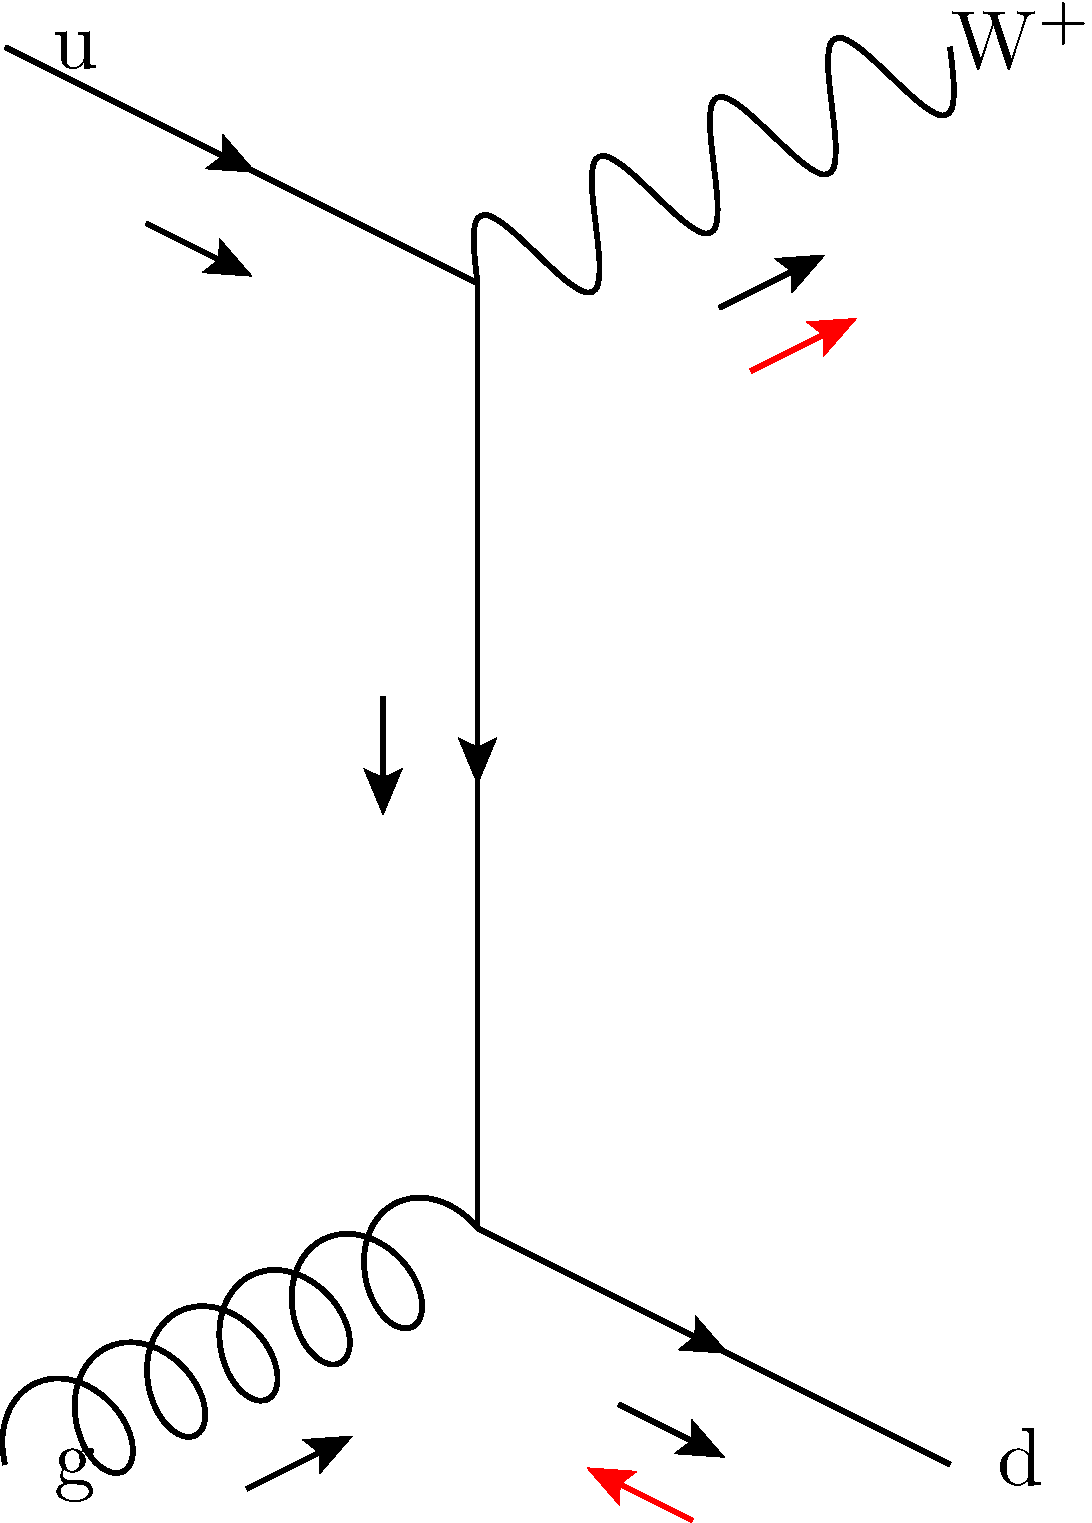
\includegraphics[width=0.25\textwidth]{fig/wpol_1jet_t}}
\caption[Diagrams showing the $\Pup\Pgluon\longrightarrow\PWp\Pdown$
subprocess]{Diagrams showing the $\Pup\Pgluon\longrightarrow\PWp\Pdown$
  subprocess in the \subref{fig:w1jet_st_s} $s$ and \subref{fig:w1jet_st_t} $t$
  channels. The black displaced arrows indicate the particle momenta. For the
  $s$ channel diagram, the helicity vectors are shown as red arrows, for the
  case of a right-handed \PW boson.}
\label{fig:w1jet_st}
\end{figure}

Writing the amplitudes of the subprocesses in \eqn~\ref{eqn:w1jet_processes}
in terms of spinor products, two distinct expressions emerge,

\begin{eqnarray*}
\mathcal{A}^{\textrm{tree}}_{(a)} &\propto&
\frac{\left<\Pdown\nu\right>^2}{\left<\Pup\Pgluon\right>\left<\Pgluon\Pdown\right>}\\
\mathcal{A}^{\textrm{tree}}_{(b)} &\propto&
\frac{\left[\Pup\Pe\right]^2}{\left[\Pup\Pgluon\right]\left[\Pgluon\Pdown\right]},
\end{eqnarray*}
where factors common to both expressions are not shown. The corresponding
cross-sections are
\begin{equation}
\label{eqn:w1jet_xs}
d\sigma^{\textrm{LO}}_{(a)} \propto (k_{\Pdown} \dot k_{\Pneutrino})^2 \quad
d\sigma^{\textrm{LO}}_{(b)} \propto (k_{\Pup} \dot k_{\Pe})^2,
\end{equation}
where the $k$ are Lorentz vectors representing the particle momenta. For each
subprocess, the helicity configurations corresponding to $(a)$ and $(b)$ are
shown in the upper and lower rows of \fig~\ref{fig:w1jet_modes}
respectively. The red arrows indicate particle helicity, with a double-stemmed
arrow for the \PW momentum. In the cases where the \PW is neither purely
left-handed nor right-handed, the arrow is placed at an angle.

Starting with the subprocess $\Pup\Pgluon\longrightarrow\PWp\Pdown$, the $(a)$
expression in \ref{eqn:w1jet_xs} correlates the axis of the \Pdown quark with
the neutrino (see \fig~\ref{fig:w1jet_modes_1a}). Due to the \VminusA
coupling, the neutrino must have a left-handed helicity and, via angular
momentum conservation, so too the \PW. The angular dependence is
$(1-\cos\tilde{\theta}^*)^2$ where $\tilde{\theta^*}$ is the angle of the
charged decay lepton with the \PW flight direction in the centre-of-mass
frame. In contrast, considering an identical particle configuration but with
helicities corresponding to $(b)$ (\fig~\ref{fig:w1jet_modes_1b}), the
\Ppositron direction is now correlated with the incoming beam
direction. Boosting to the \PW rest frame, at high \PtW, the incoming quark and
gluon are nearly parallel and, given a scattering angle of 90\degrees, the \Pup
quark momentum is seen to be half that of the \Pdown quark. The angular
dependence is thus $\frac{1}{4}(1+\cos\tilde{\theta}^*)^2$ yielding a
right-handed polarisation at a quarter of the rate of the left-handed component.

For the sub-dominant process $\Pup\APdown\longrightarrow\PWp\Pgluon$, the terms
in \eqn~\ref{eqn:w1jet_xs} correlate the momenta of the decay leptons with the
beam direction. The two cases are shown in \figs~\ref{fig:w1jet_modes_2a} and
\ref{fig:w1jet_modes_2b}. Although it can be seen once again that a left-handed
and right-handed polarisation emerge, in this case they are found to cancel for
a scattering angle of 90\degrees and thus give no net polarisation. Lastly, for
the subprocess $\Pgluon\APdown\longrightarrow\PWp\APup$, show in
\figs~\ref{fig:w1jet_modes_3a} and \ref{fig:w1jet_modes_3b}, the $(b)$
contribution correlated the \Pup quark with the \Ppositron direction, leading to a
dominantly right-handed polarisation. However, since the \ac{PDF} $\APdown(x)$
is much smaller than $\Pup(x)$, this effect is largely washed out by the
dominant left-handed polarisation mode.

\begin{figure}
\centering
\subfloat[]{\label{fig:w1jet_modes_1a}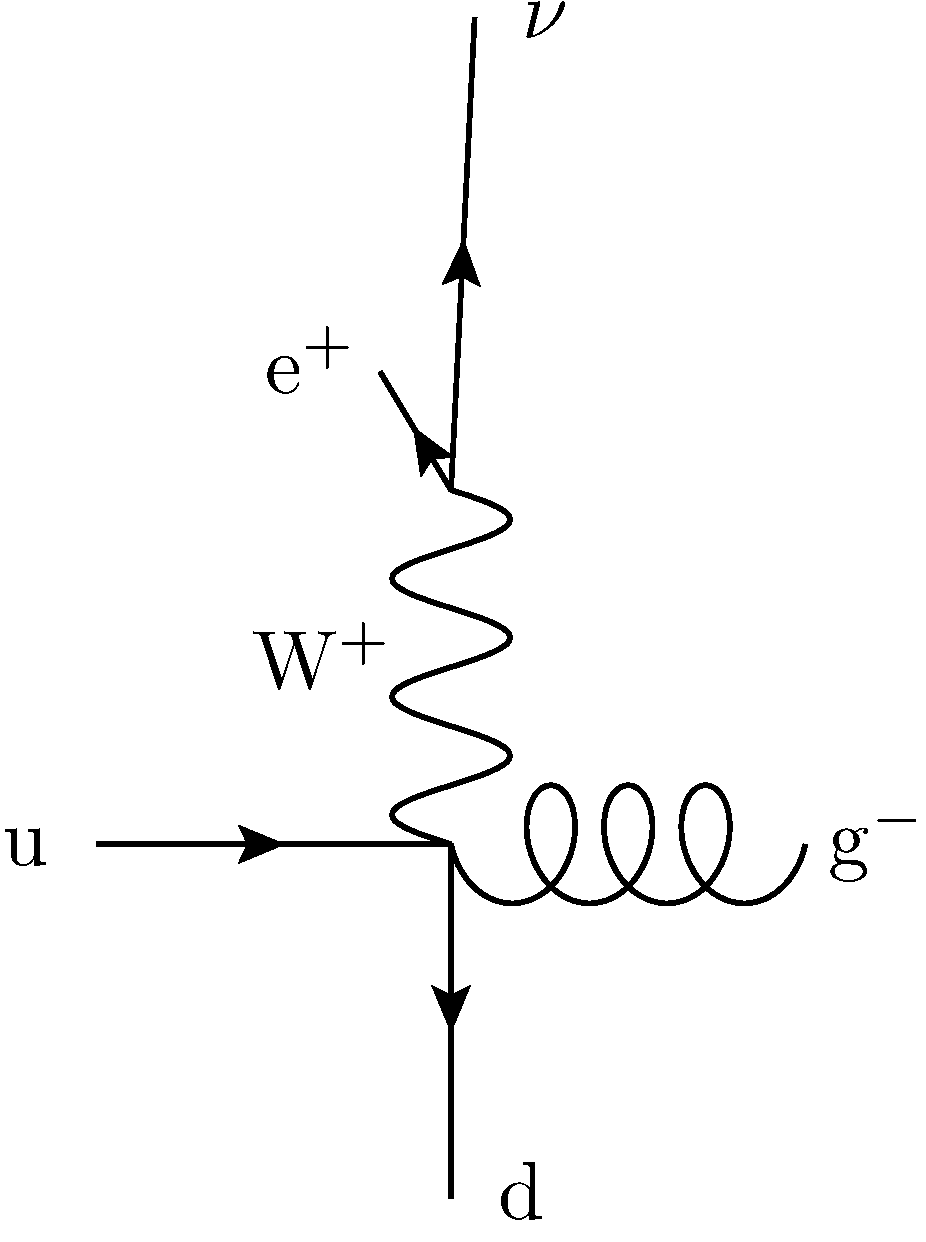
\includegraphics[width=0.3\textwidth]{fig/wpol_prod_a}}\quad
\subfloat[]{\label{fig:w1jet_modes_2a}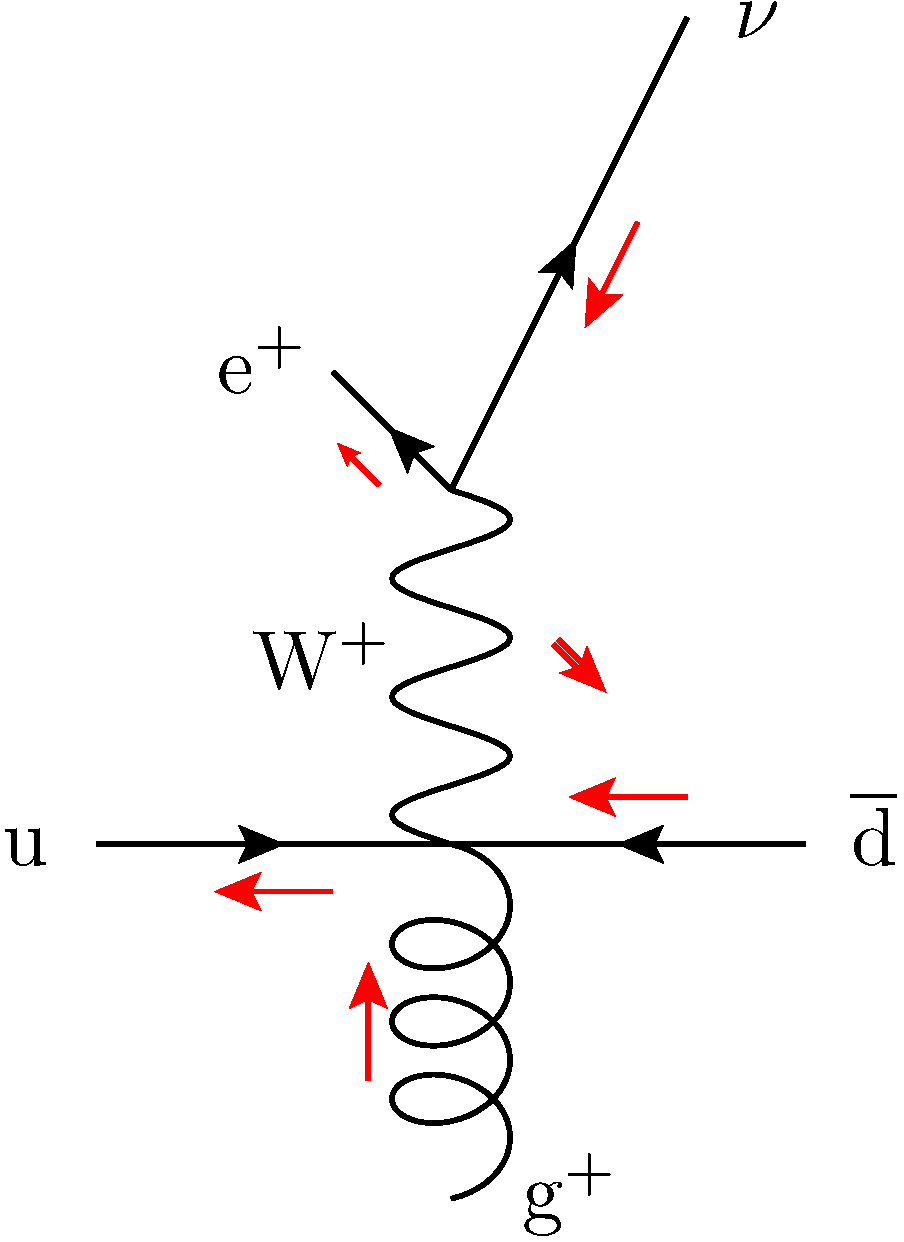
\includegraphics[width=0.3\textwidth]{fig/wpol_prod_b}}\quad
\subfloat[]{\label{fig:w1jet_modes_3a}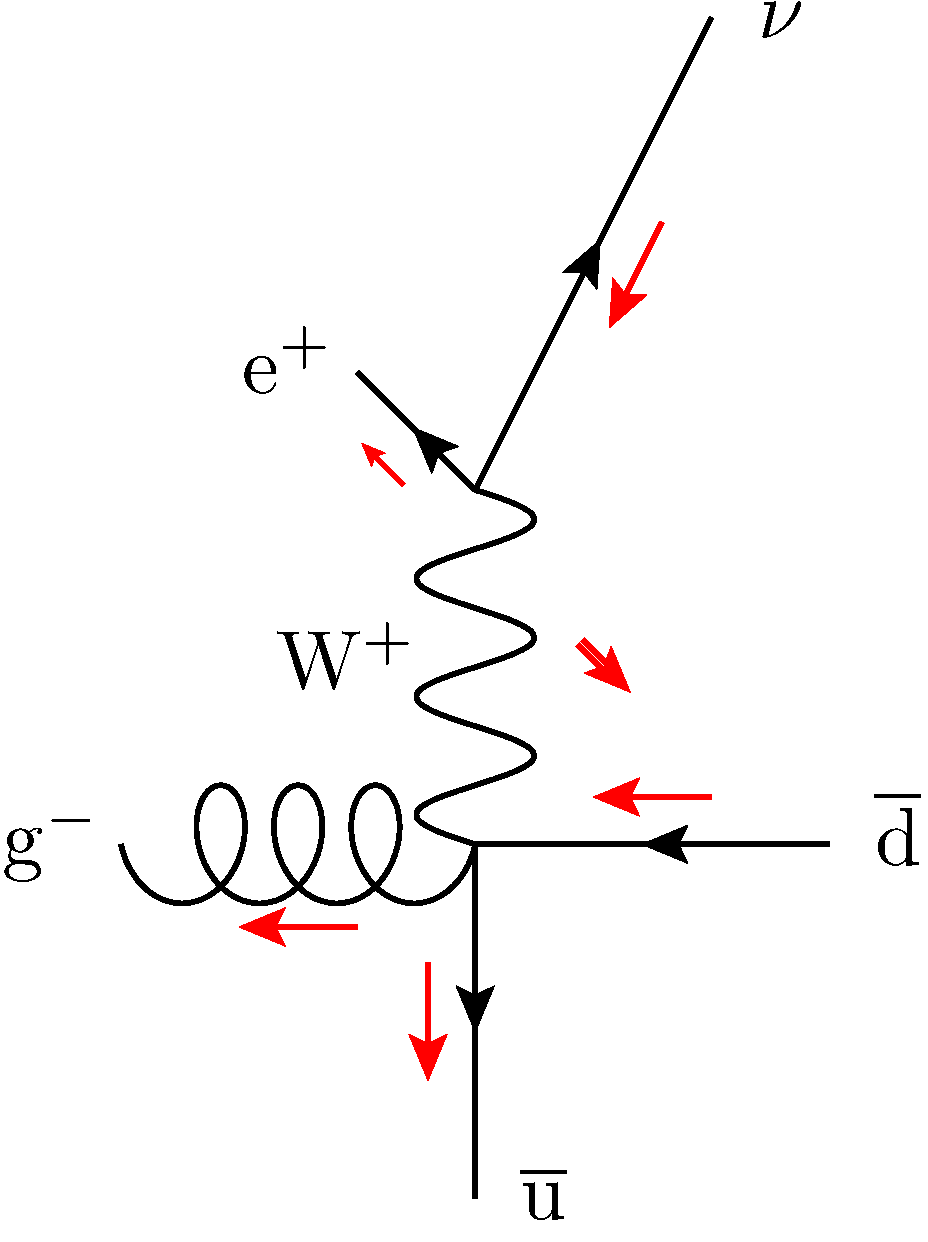
\includegraphics[width=0.3\textwidth]{fig/wpol_prod_c}}\\
\subfloat[]{\label{fig:w1jet_modes_1b}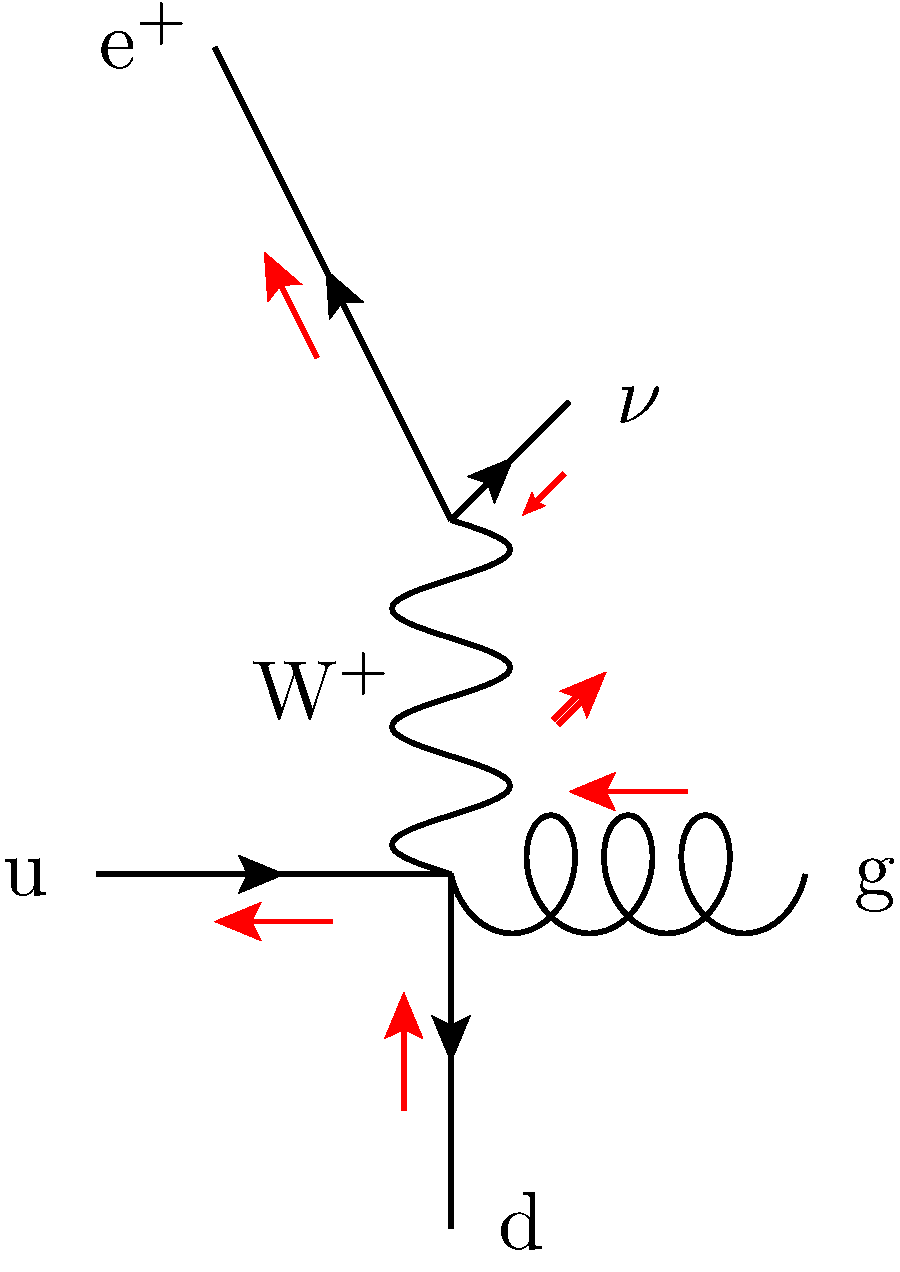
\includegraphics[width=0.3\textwidth]{fig/wpol_prod_d}}\quad
\subfloat[]{\label{fig:w1jet_modes_2b}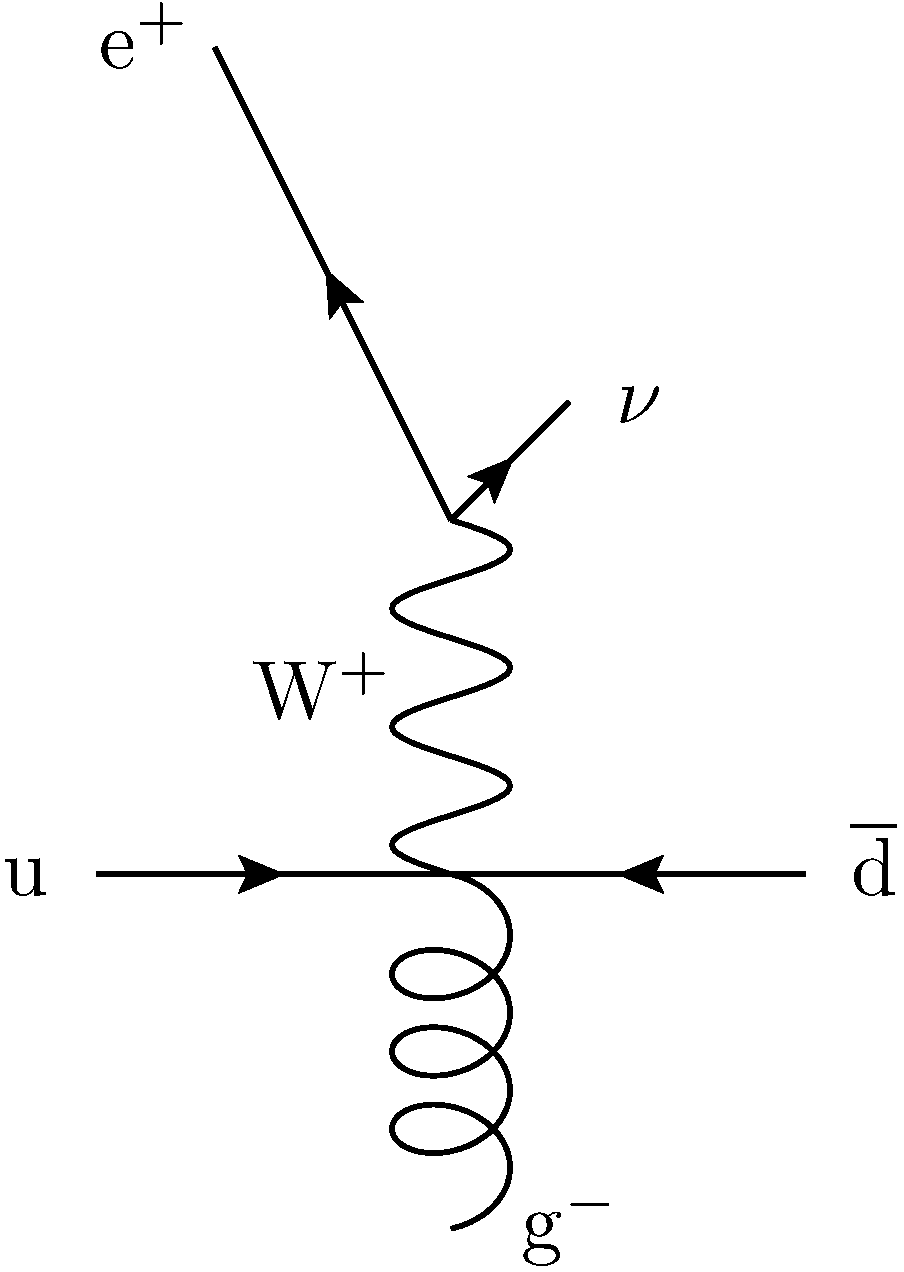
\includegraphics[width=0.3\textwidth]{fig/wpol_prod_e}}\quad
\subfloat[]{\label{fig:w1jet_modes_3b}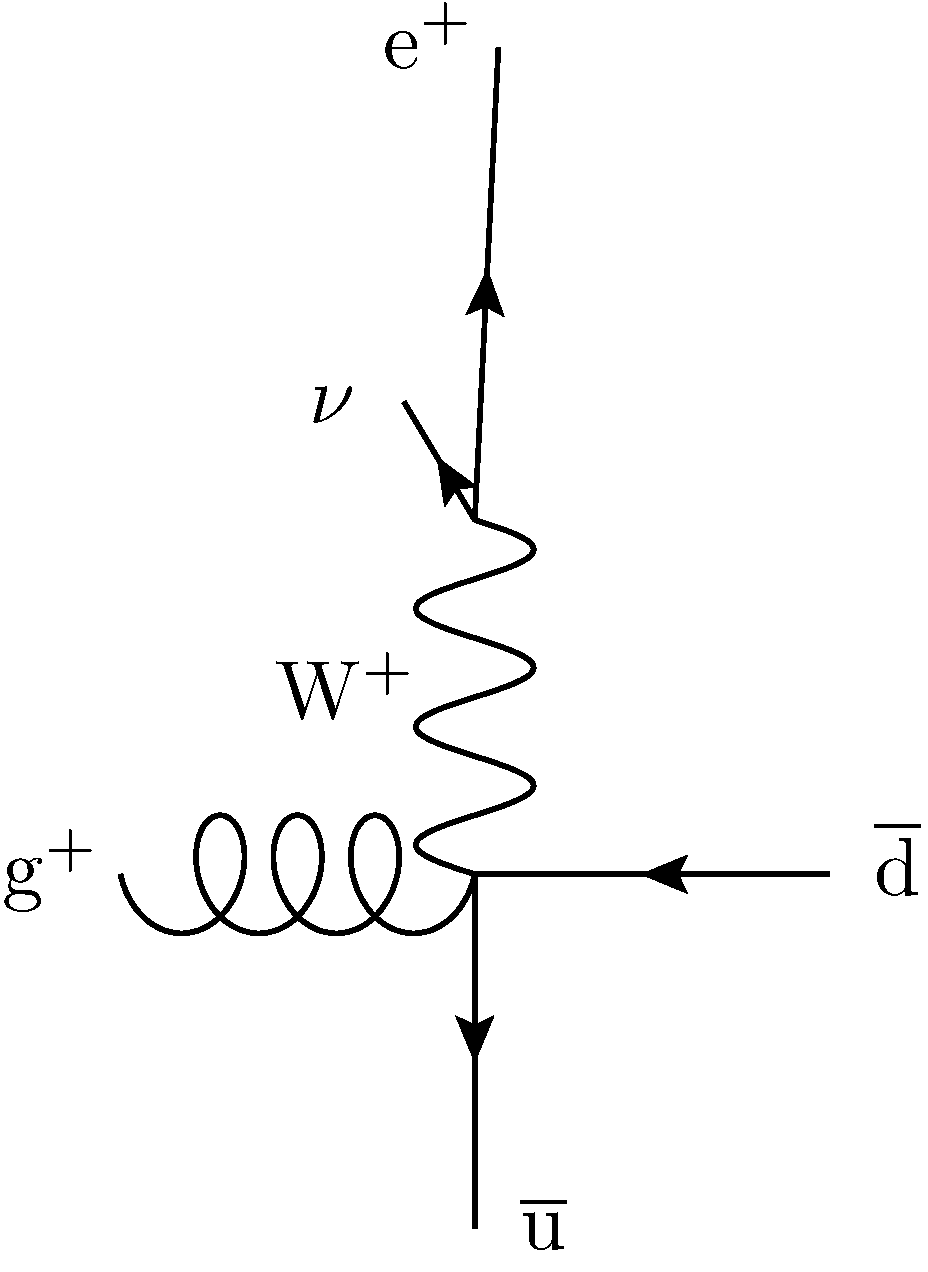
\includegraphics[width=0.3\textwidth]{fig/wpol_prod_f}}
\caption{Illustrations of $\PWplus+1$~jet production modes at the LHC. The
  gluon superscript indicates its helicity}
\label{fig:w1jet_modes}
\end{figure}

As has been seen, the proton-proton environment at the \ac{LHC} is expected to
lead to a dominance of left-handed over right-handed helicity states for \PW
bosons with large transverse momentum. In the next section, theoretical
background related to helicity measurement will be presented.

\subsection{Studying Helicity}

\subsubsection{The Helicity Frame}
The polarisation effects may be conveniently studied within the helicity frame
of the \PW boson. This is defined as the rest frame of the \PW with the
polarisation axis (here, the z-axis) is aligned along the line of flight of the
\PW in the lab frame. The x-axis is then chosen to lie along the plane spanned
by the two colliding protons in the boson rest frame with the sense chosen such
that the angle between it and the nearest proton is minimised. The y-axis is
then fixed to be perpendicular to these two (the coordinate system is
right-handed). The polar angle, \thetastar is measured in the $y-z$ plane
between the positive z-axis and the lepton. Likewise, the azimuthal angle,
\phistar is measured in $x-z$ between the positive $x$ axis and the lepton. This
arrangement is illustrated in \fig~\ref{fig:wpol_helicity_frame}. For $0 <
|\phistar| < \frac{\pi}{2}$, the charged lepton will have a larger rapidity that
the \PW boson and thus a smaller \Pt. Alternatively, for $\frac{\pi}{2} <
|\phistar| < \pi$, the lepton will have a smaller rapidity and a larger \Pt.

\begin{figure}[ht!]
%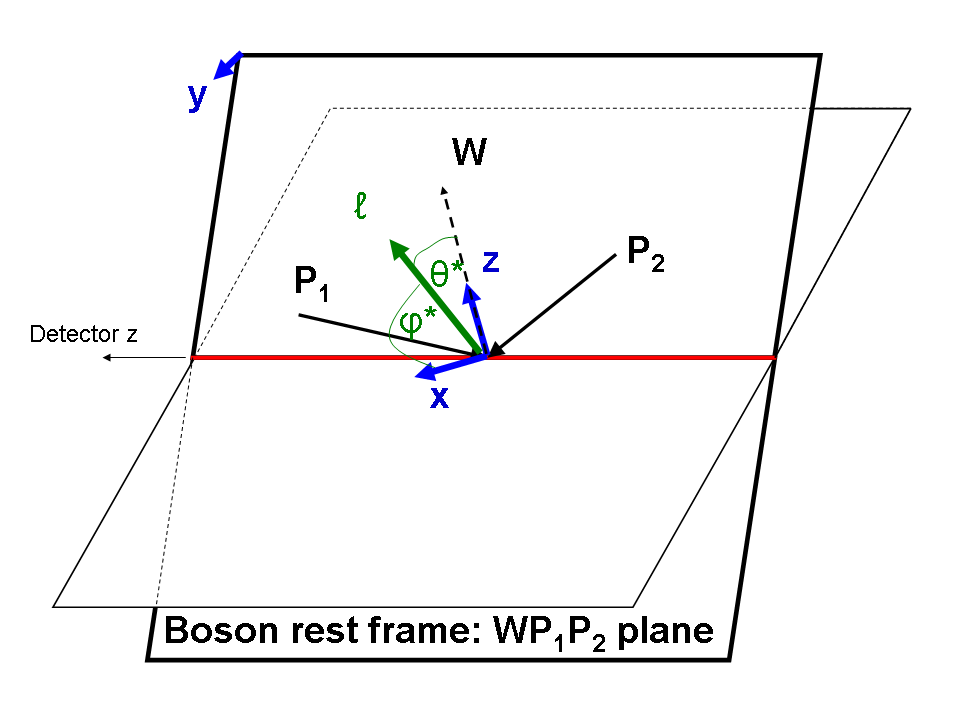
\includegraphics[width=0.8\textwidth]{fig/helicity_frame_polnote}
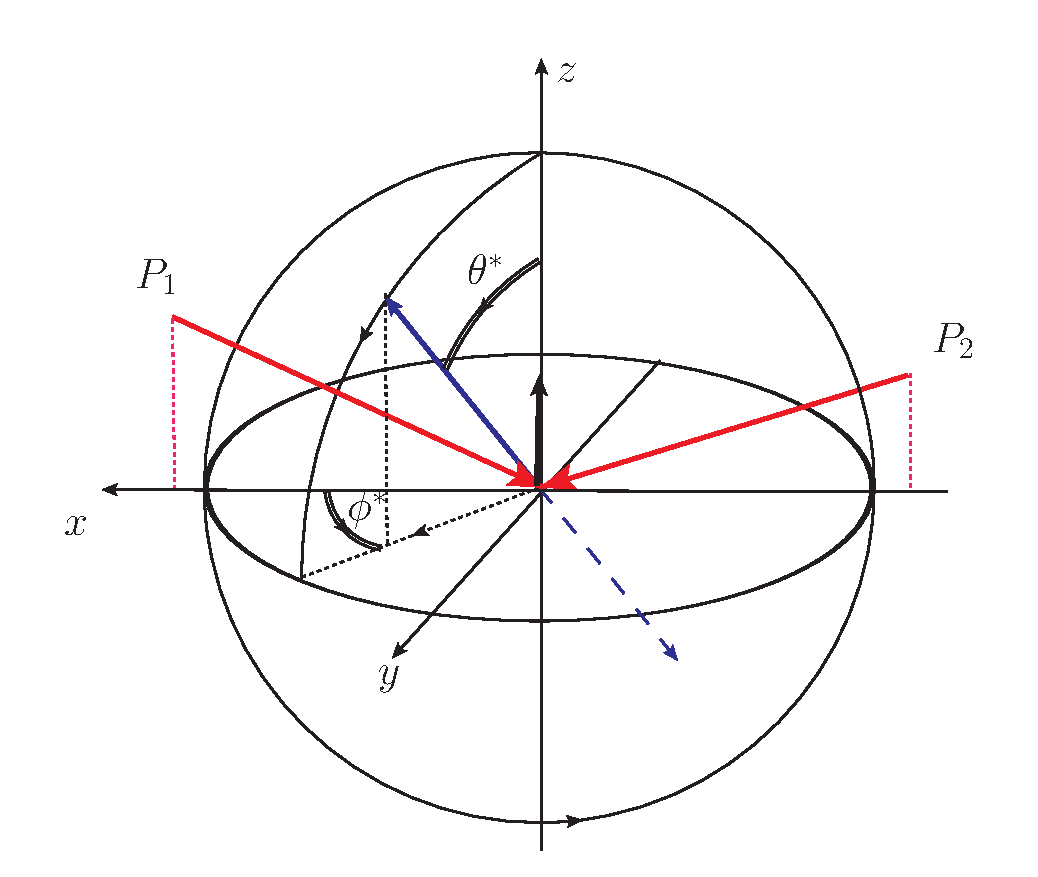
\includegraphics[width=0.8\textwidth]{fig/helicity_frame_better}
\caption[The Helicity Frame]{The Helicity Frame~\cite{berger_left_handed_w}}
\label{fig:wpol_helicity_frame}
\end{figure}

\subsubsection{Quantifying Helicity}
\label{sec:quant_helicity}
The hadronic cross-section of the \PW is obtained within the parton model by
weighting the individual parton-level cross-sections by the respective parton
densities~\cite{mirkes_w_1994},
\begin{equation*}
\frac{d\sigma^{h_1 h_2}}{d(\PtW)^2 dy d\Omega^*} = \sum_{ab} \int dx_1 dx_2
f_a^{h_1}\left(x_1, \mu_F^2\right)f_b^{h_2}\left(x_2, \mu_F^2\right)
\times \frac{s d\tilde{\sigma}_{ab}}{dt du d\Omega^*} \left(x_1 P_1, x_2 P_2,
\alpha_s (\mu_R^2)\right),
\end{equation*}
where $h_1$ and $h_2$ are the interacting hadrons and the sum runs over $a,b =
\Pquark, \APquark, \Pgluon$. The \acp{PDF} $f_a^{h}\left(x, \mu^2\right)$ give
the probability of finding a parton $a$ with momentum fraction $x$ in hadron $h$
when probed at a scale $\mu^2$. The $d\tilde{\sigma}_{ab}$ are the parton-level
cross-sections for the chosen process(es). The hadron-level Mandelstam variables
are written uppercase,
\begin{equation*}
S = (P_1 + P_2)^2 \qquad T = (P_1 - Q)^2 \qquad U = (P_2 - Q)^2,
\end{equation*}
and parton-level lowercase,
\begin{eqnarray*}
s &=& (p_1 + p_2)^2 = x_1 x_2 S\\
t &=& (p_1 - Q)^2  = x_1(T-Q)^2 +Q^2\\
u &=& (p_2 - Q)^2 = x_2(U -Q)^2 + Q^2,
\end{eqnarray*}
and
\begin{equation*}
p_1 = x_1 P_1 \qquad p_2 = x_2 P_2.
\end{equation*}
This can be rewritten in terms of a standard set of angular coefficient $A_i$,
to give~\cite{mirkes_w_1992}
\begin{align}
\label{eqn:wpol_diff_xs}
\frac{d\sigma}{d(\PtW)^2 dy d\cos\theta d\phi} = \frac{3}{16\pi}
\frac{d\sigma^{-1}}{d(\PtW)^2 dy} &\left [ \left(1+\cos^2\theta\right) \right. \nonumber\\
 &+ \frac{1}{2} A_0 \left ( 1 - 3\cos^2\theta \right ) + A_1 \sin 2\theta\cos\phi \nonumber\\
 &+ \frac{1}{2}A_2\sin^2\theta\cos 2\phi + A_3\sin\theta\cos\phi \nonumber\\
 &+ A_4\cos\theta + A_5\sin^2\theta\sin 2\phi \nonumber\\
 &+ A_6\sin 2\theta\sin \phi + A_7\sin\theta\sin\phi
\end{align}

% TODO: Figure out the difference between  theta and theta*
The $A_i$ are ratios of the separate helicity cross-sections of the boson to its
total unpolarised cross-section and are dependent on the \PW boson charge,
transverse momentum \PtW and rapidity \YW. \eqn~\ref{eqn:wpol_diff_xs} can be
integrated over $\phi$ and \PtW to give:
\begin{equation}
\label{eqn:wpol_xs_Ai}
\frac{d\sigma}{d\cos\theta} \propto \left(1+\cos^2\theta\right) +
\frac{1}{2}A_0\left(1-3\cos^2\theta\right) + A_4\cos\theta.
\end{equation}

% TODO: Check all this bs!
Due to the \VminusA nature of the Electroweak theory, the \PWp (\PWm) may couple
only to left-handed (right-handed) fermions and right-handed (left-handed)
anti-fermions, therefore the angular momentum state of the decay leptons is
\begin{eqnarray*}
\ket{\Pl\Pgn^{J,M}} &=& \ket{\frac{1}{2}, \pm \frac{1}{2}}
\oplus \ket{\frac{1}{2}, \pm\frac{1}{2}} \\
&=& \textrm{either}\quad\ket{1, +1}\quad\textrm{or}\quad \ket{1, -1},
\end{eqnarray*}
where $\ket{J, M}$ represents an angular momentum state with a total angular momentum $J$ and projection $M$.

Rotating these states through the angle \thetastar,
\begin{equation}
\ket{\Pl\Pgn^{J,M}}' = \sum_{M'=-J}^{M'=+J} d_{M, M'}^J \ket{J, M'}.
\end{equation}
The angular momentum of a \PW boson in a helicity eigenstate is then
$\ket{\PW^{J,M''}}$. The matrix element for the angular momentum coupling can be
written
\begin{eqnarray*}
\braket{\PW^{J,M''}}{\Pl\Pgn^{J,M}}' &\sim& \sum_{M'=-J}^{M'=+J} d_{M M'}^{J}
\braket{J,M''}{J,M'} \\
&\sim& d^{J}_{M M''} \braket{J,M''}{J,M''} \sim d_{M M''}^{J}.
\end{eqnarray*}
To calculate the cross-section, square the matrix elements and sum over the
helicity states ($M''$) of the incoming $\PW$, weighting each state by the helicity
fraction $f_{M''}$,
\begin{equation*}
\sigma(\PW\longrightarrow\Pl\Pgnl) \sim f_0 \left|d_{M 0}^1\right|^2 + f_{-1} \left|d_{M
    -1}^1\right|^2 + f_{1} \left|d_{M +1}^1\right|^2.
\end{equation*}
Where $f_0 + f_1 + f_{-1} = 1$. Finally, using the fact that for \PWpm, $M=\pm1$
and replacing for the elements of the D-matrices in terms of $\cos\thetastar$
gives,
\begin{equation}
\label{eqn:wpol_helicity_fractions}
\sigma(\thetastar_{\Plpm}) = \frac{\f0}{2}\sin^2\thetastar_{\Plpm} +
\frac{\fL}{4} \left(1\mp\cos\thetastar_{\Plpm}\right)^2 +
\frac{\fR}{4} \left(1\pm\cos\thetastar_{\Plpm}\right)^2.
\end{equation}
Note that the helicity fractions \ffi have been relabelled to give a more
intuitive interpretation as the left-handed, right-handed and longitudinal
helicity fractions. Comparing now to \eqn~\ref{eqn:wpol_xs_Ai}, we identify
\begin{eqnarray*}
A_0 \sim f_0\\
A_4 \sim \pm \fLmfR.
\end{eqnarray*}
Whilst the $A_i$ are the more fundamental parameters from a theoretical point of
view, the helicity fractions \f0, \fL and \fR will sometimes be more convenient
for experimental discussions. The other \Ai parameters will mostly not be
discussed, though their small effect on the measurement will be evaluated.

In \chap~\ref{sec:polarisation}, the measurement of the helicity fractions
\fL, \fR and \f0 will be described. The primary intention is to confirm the
prediction that the left-handed mode dominates at high \PtW, or equivalently,
$\fLmfR > 0$. It is also expected that $\fL > \f0$.

The evolution of the polarisation fractions with \PtW has also been
studied~\cite{berger_left_handed_w}. The evolution of \fL, \fR and \f0 for the
\PWp is shown in \fig~\ref{fig:framework_ptw}. Firstly, the increase of \fLmfR
with \PtW can be seen. Secondly, because of the equivalence
theorem~\cite{equiv_theorem,tev_physics,gounaris,cornwall,elementary_pp}, the
longitudinal mode behaves as the corresponding Goldstone boson (see
\sec~\ref{sec:sm_goldstone}) at large \PtW. This leads to the dip in \f0.

Whilst the dependence on \PtW make for a very interesting measurement, it was
found to be infeasible with the relatively small data sample used for this
analysis.

\begin{figure}[h]
\centering
\subfloat[\fL]{\label{fig:framework_ptw_fL}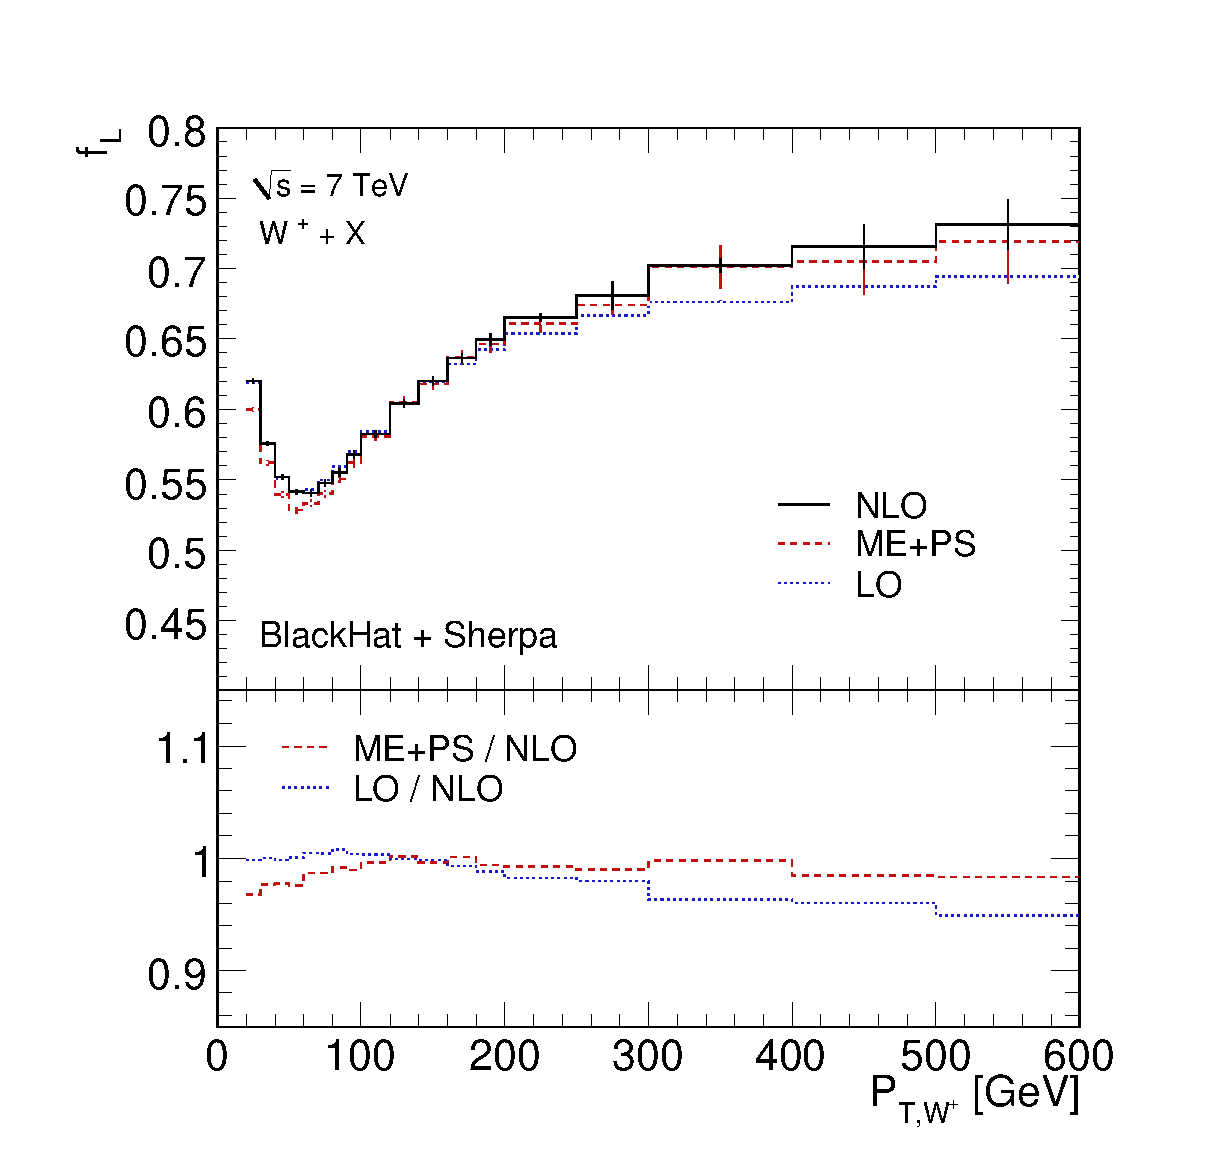
\includegraphics[width=0.29\textwidth]{fig/fL_Wp}}
\subfloat[\fR]{\label{fig:framework_ptw_fR}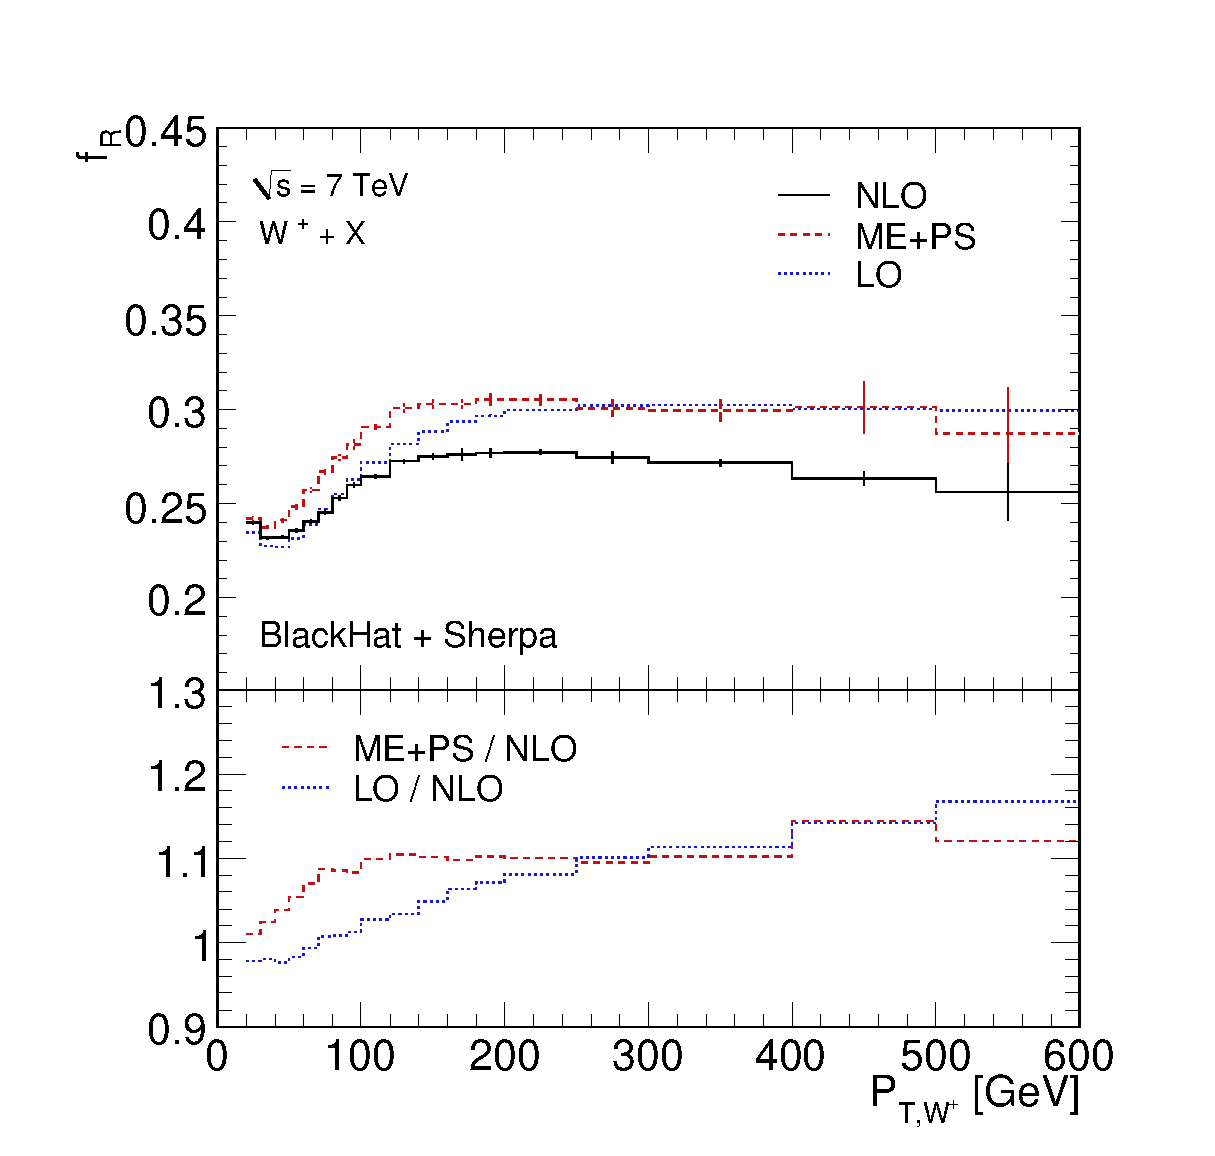
\includegraphics[width=0.29\textwidth]{fig/fR_Wp}}
\subfloat[\f0]{\label{fig:framework_ptw_f0}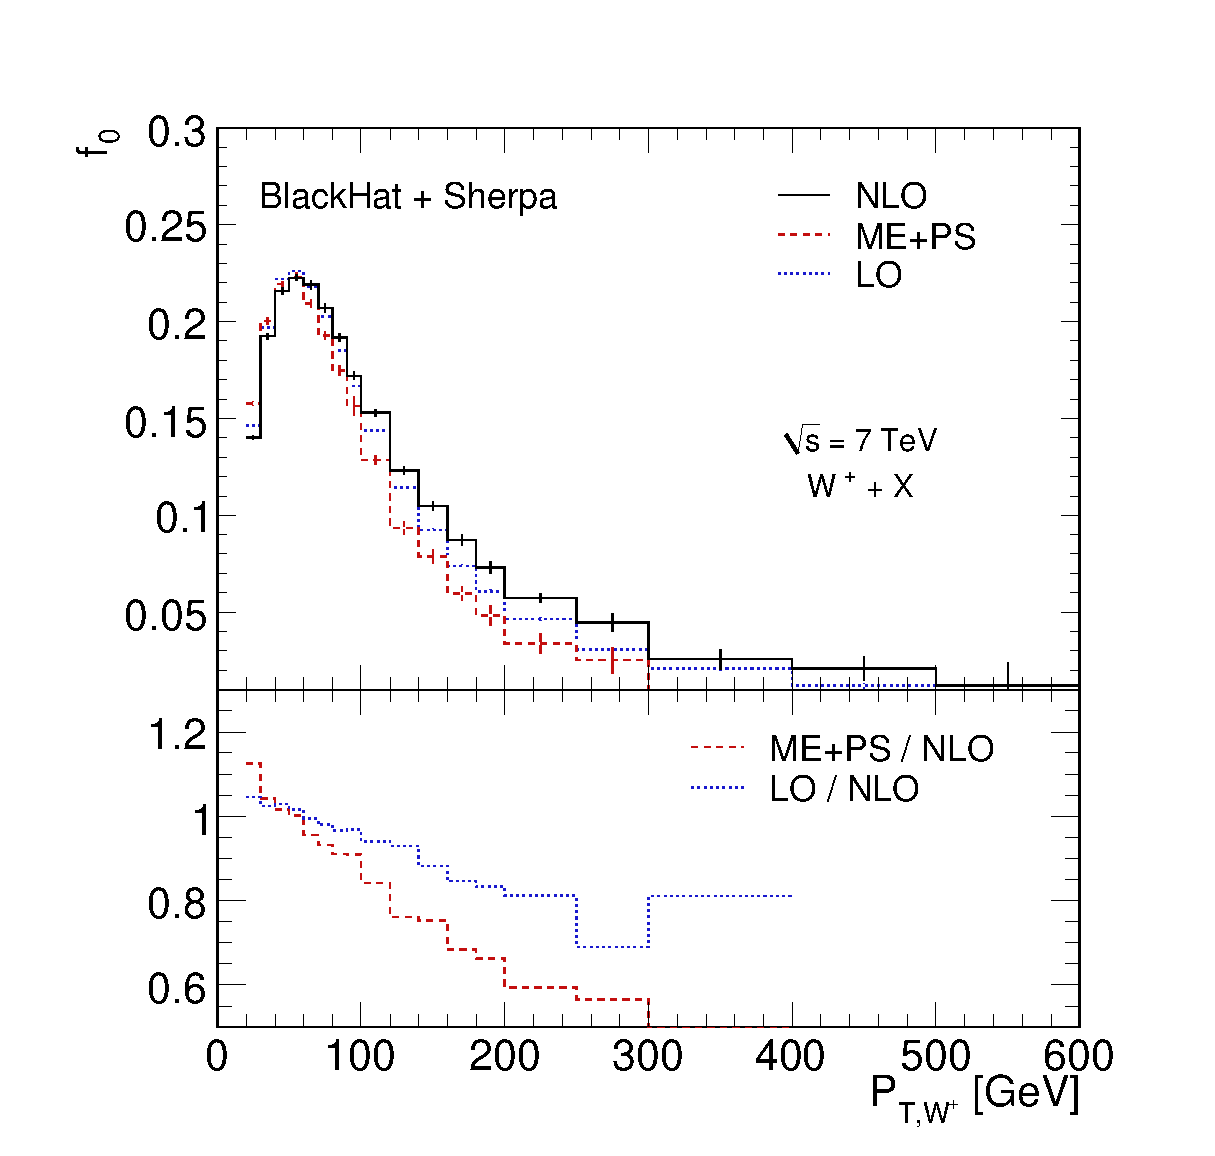
\includegraphics[width=0.29\textwidth]{fig/f0_Wp}}
\caption{The polarisation fractions \fL, \fR and \f0 as a function of \PtW for
  \PWp production are shown in the upper panes of
  \figs~\ref{fig:framework_ptw_fL}, \ref{fig:framework_ptw_fR} and
  \ref{fig:framework_ptw_f0} respectively. Three predictions are shown: the
  fixed-order \ac{NLO} result as a solid black line, the \ac{ME+PS} result as
  red dashed line and the fixed-order \ac{LO} result as a dotted blue
  line. Uncertainties are indicated by thin vertical lines. The lower pane in
  each plot show the ratio of each prediction with respect to the \ac{NLO}
  prediction~\cite{berger_left_handed_w}.}
\label{fig:framework_ptw}
\end{figure}

\section{Modelling New Physics}
\label{sec:framework_susy}
\subsection{\acl{CMSSM}}
\label{sec:cmssm}
It was said in \chap~\ref{sec:susy} that the \ac{MSSM} is problematic
from the point of view of collider searches due to the extremely large number of
parameters associated with supersymmetry breaking. In order to make quantitative
statements about the sensitivity of a given experimental search, a more
restricted theory must be considered.

One such theory that has often been used is the \ac{CMSSM}. The \ac{CMSSM} is
inspired by \ac{mSUGRA}~\cite{kane_minimal}. This proposes a
gravity-mediated \ac{SUSY} breaking mechanism via a hidden sector. This
assumption reduces the parameter space of the \ac{MSSM} to just 5 parameters, 4
of which are continuous:
\begin{itemize}
\item a universal trilinear scalar coupling, $A_0$;
\item a single scalar mass, $m_0$;
\item a single gaugino mass, $m_{\frac{1}{2}}$;
\item $\tan\beta$ where $\beta$ is the ratio of the Higgs' vacuum expectation values and
\item $sign \mu$ where $\mu$ is the self-coupling of the Higgs field.
\end{itemize}

Whilst this proves to be a much more useful model from the point of view of
experimental searches, there is no particular reason to assume that \ac{SUSY} is
broken in this way. The restricted parameter space of the \ac{CMSSM} may
disfavour a number of topologies which would appear in a larger class of
\ac{SUSY} theories. An additional, but related difficulty is that
interpretations of results within the \ac{CMSSM} may not be robustly
extrapolated to alternative models. As will be seen, both of these difficulties
are addressed by a more generic set of \ac{SUSY} inspired models. These will be
presented in the next section.

\subsection{Simplified Models}
\label{sec:sms}
It is often the case that theorists, having devised some theory, and made
concrete phenomenological predictions from it, wish to test it against
experimental data. The difficulty then arises of taking these predictions and
translating them into a form where they can be compared directly with
experimental results. Typically, these results will be provided in the form of
one or more event yields, corresponding background predictions and statistical
and systematic uncertainties. In some (but probably not most) cases, the
relevant correlations will also be included. The theorist must then take the
predictions of the theory and apply experimental resolution effects to them in
order to simulate the expected signal yield. Modern detectors are highly complex
and require very complex simulation to precisely model all of the resolution and
acceptance effects. In some cases, in particular for relatively simple kinematic
quantities, a simplified parameterisation may suffice. However, detailed checks
will be required to confirm that a given approximation reproduces, with adequate
fidelity the results of the full detector simulation or the actual recorded
data. If it can be confirmed that this is the case, the theorist may then
proceed to redo the work of the experimentalist in modelling the various
statistical and systematic effects in the form of a likelihood
function. Finally, they may then utilise all of these components to produce
their own statistical interpretation of the data against the chosen theory.

Clearly, this procedure is both laborious and error-prone. It was therefore
proposed that the \ac{LHC} experiments would provide a richer interpretation in
the context of a set of ``Simplified Models''. Broadly speaking, a simplified
model is a highly simplified effective theory, chosen to characterise a
particular phenomenological scenario present within one or more \ac{NP}
models. Free parameters which have little effect on the physics (at least at
small integrated luminosities) are integrated out, leaving only those which a
greater effect on the physics. In constructing a number of these models, the
full space of possibly physical signatures arising in much more complicated
theories may be spanned. This is sometimes referred to as a \acf{SMS}

Although the concept of a simplified model is quite general, the discussion here
will focus on those inspired by \ac{SUSY} or ``\ac{SUSY}-like'' theories, and
more specifically those relevant to the single-leptonic experimental search
described in previous chapters. As will be seen in the next section, these offer
a much richer set of phenomenologies than those allowed in the \ac{CMSSM}.

% \todo[size=\tiny, linespacing=0.5]{Mention that SMS are used for characterisation of discovery as well as
%   design of searches}

\subsubsection{Dark Matter Models}
As discussed in \chap~\ref{sec:susy}, a highly desirable prediction of certain
supersymmetric theories is the existence of a stable, weakly-interacting
particle or \ac{WIMP}. This is a dark matter candidate with a striking
experimental signature at collider experiments -- a large missing energy
component in the transverse plane. At hadron colliders, the initially produced
particles are likely to be coloured (either squarks or gluinos). These will then
decay, either directly or via a cascade to a \ac{WIMP}.

Since these topologies are largely inspired by \Rparity conserving \ac{SUSY},
similar terminology and notation will be used to refer to their particle
content. This should not be taken to suggest that these topologies are exclusive
to \ac{SUSY} type theories. For instance, the mass splittings between the
constituent particles are allowed to be much larger than for the \ac{CMSSM}.
%\cite{interpretation_pas}.

The topologies considered here can be split into two categories. The first
begins with pair-production of a neutral, coloured object -- the gluino in the
case of \ac{SUSY}. The second is initiated by production of a charged, coloured
object -- the squark in \ac{SUSY} . As for the \ac{CMSSM}, these are expected to
be produced most abundantly at the \ac{LHC}.

In either case, the squark or gluino type particle then decays, either directly
to an \ac{LSP} or via some intermediate particles (comparable to the heavy
electroweakinos of \ac{SUSY}) -- a cascade decay.
% The naming convention adopted here gives each model a name, T$x$. For models
% resembling pair production of the gluinos, $x$ will be an odd integer and for
% those representing squark production, an even integer. For gluino-type
% topologies, $x$ values of 1, 3 and 5 represent respectively: direct decay of
% both particles, one cascade and one direct decay and two cascade decays. The
% squark-type models are similarly labelled 2, 3 and 4 representing the same
% combinations of direct and cascade decays.

\begin{figure}
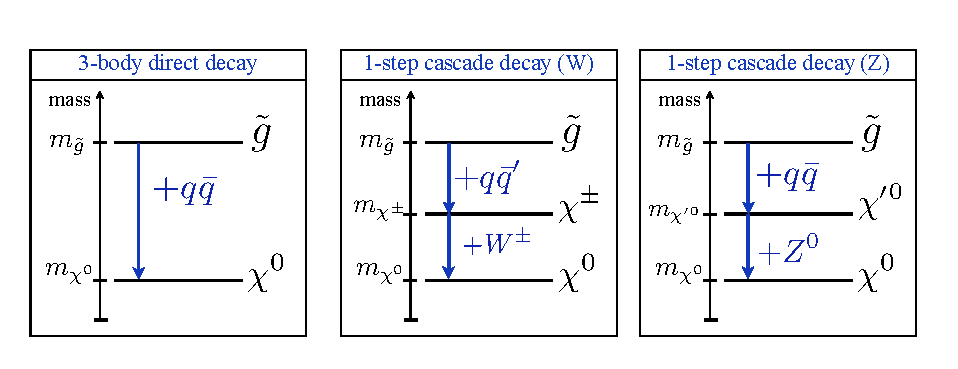
\includegraphics[width=\textwidth]{fig/gluino_sms_decays}
\caption{Illustration of direct and cascade gluino decay modes within \ac{SUSY}
  simplified models.~\cite{alves_simplified_2011}}
\label{fig:gluino_sms_decays}
\end{figure}

\subsubsection{Connection to Supersymmetry}
Considering first the gluino pair-production models
(\fig~\ref{fig:gluino_sms_decays}), we shall assume that the squarks are heavier
and therefore kinematically inaccessible. If this were not the case, the
phenomenology would be better described by the squark-type models.

In such supersymmetric models, the gluino may decay only via an off-shell
squark~\cite{alwall_simplified}. This may be either directly to the LSP or
indirectly via intermediate states. Direct decays correspond to \ac{SUSY}
scenarios where either~\cite{alves_simplified_2011}:
\begin{itemize}
\item $\PSgxzi \approx \PSB$ and the $\PSq_{R}$ are lightest or the $\PSW$ is kinematically
  inaccessible;
\item $\PSgxzi \approx \PSW$ and either $\PSq_{L}$ are lightest or there is no
  splitting between the left and right-handed squarks and
\item $\PSgxzi \approx \PSH$ and either heavy-flavour squarks are inaccessible or
  $\PSB$ and $PSW$ are inaccessible.
\end{itemize}

This is not generally true in either \ac{mSUGRA} or \ac{GMSB} but does
correspond to certain \ac{AMSB} scenarios~\cite{alves_simplified_2011}.

Alternatively, the gluino may undergo a cascade decay via an intermediate mass
state, either a chargino or a heavy neutralino. This will subsequently decay to
the \ac{LSP} via either a $\PW$ or a $\PZ$ boson.

The situation is similar in the case of squark pair-production, except that in
the without the intermediate off-shell squark, the jet multiplicity is reduced.

\subsubsection{Single Lepton Topologies}
To provide a meaningful interpretation of the single lepton search detailed in
\chap~\ref{sec:susysearch}, two simplified models have been chosen from the
range presented above. The models, \TthreeW and \Ttwott, have been chosen in
particular since they offer topologies which are likely to enter the selection
of a single lepton \ac{SUSY} search.

\begin{figure}[h]
\centering
\subfloat[]{\label{fig:sms_topologies_t3w}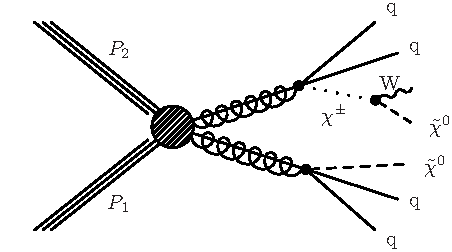
\includegraphics[width=0.45\textwidth]{fig/T3w}}\quad
\subfloat[]{\label{fig:sms_topologies_t2tt}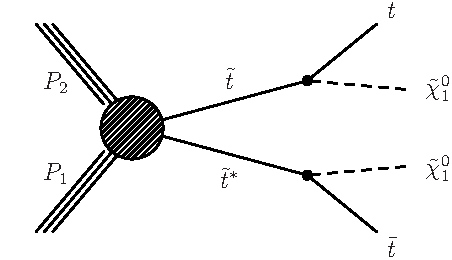
\includegraphics[width=0.45\textwidth]{fig/T2tt}}
\caption[Illustration of two simplified model topologies suited to a single
lepton supersymmetry search]{Illustration of two simplified model topologies
  suited to a single lepton supersymmetry search:
  \subref{fig:sms_topologies_t3w} \TthreeW and \subref{fig:sms_topologies_t2tt}
  \Ttwott~\cite{susy_interpretation_pas}}
\label{fig:sms_topologies}
\end{figure}

The \TthreeW model is a gluino pair-production model, in which one of the mother
particles undergoes a cascade decay via an intermediate particle. The $\PW$ in
the model name indicates that this intermediate particle is then ``forced'' to
decay to a \PW boson. This topology is illustrated in
\fig~\ref{fig:sms_topologies_t3w} and is seen to be similar to the example
\ac{SUSY} decay illustrated in \fig~\ref{fig:susy_1lep_decay}. This model is
parameterised by the mass of the mother particle, \Mgluino, the mass of the
daughter particle, \Mlsp and the mass of the intermediate particle, \Mchargino.

The second model, \Ttwott, begins with squark pair production with both mother
particles decaying directly to the \ac{LSP}. Furthermore, both squarks are
assumed to be stop particles -- the superpartner of the top quark -- each
decaying to a \ac{SM} top quark. This decay topology is illustrated in
\fig~\ref{fig:sms_topologies_t2tt}. Such events with two top quarks in the final
state, should give an experimental signature suitable for a single lepton
search.

The \Ttwott model reflects scenarios in which the stop is the lightest of the
squarks. These are theoretically attractive for a number of reasons
(see~\cite[{p.~202}]{sparticles} and~\cite{light_stop}). Since this does not
contain an intermediate mass state, it has only two paramters: the mass of the
mother, \Mstop and the mass of the daughter, \Mlsp.

\subsubsection{Combining Topologies}
For phenomenological purposes, each separate decay topology may be considered as
an independent simplified model. The predictions of a whole set of topologies
can then be combined by taking linear combinations. For direct comparison
against experimental data, it is desirable to simulate a desired set of
topologies within a monte-carlo generator by ``turning on'' the chosen physics
subprocesses. The model parameter space can be sampled by moving through a
lattice of values in the desired range. At each lattice site, a statistically
sufficient number of events is generated with the appropriate parameter values
inserted into the configuratxoion of the \ac{MC} generator.